%% !TEX program = xelatex
\documentclass[12pt,final]{novelette} % font size, twoside, twocolumn, draft-final, use extarticle for 8-20pt

\title{Calculus III Final 2568}
\author{Kaka Cring}
\date{\today}

% !TEX root = calculus_iii_midterm.tex
\settasks{
    label=\arabic*.,
    label-align=left,
    label-width=0.8em
}

\setlength\headheight{0pt}  % header height
\setlength\footskip{48pt}    % space before base of footer
\addtolength\textheight{40pt}
\renewcommand{\headrulewidth}{0pt} % width of header line
\fancyhead[L,R]{}
\fancyfoot[C]{\fbox{\bf หน้าที่ \thepage}}

\renewcommand{\qmark}[1]{\textit{(#1\ คะแนน)}}
\newcommand{\ansbox}{\ensuremath{\boxed{\hspace*{7em}\vphantom{\dfrac12}}} {}}
\newcommand{\ansboxs}{\ensuremath{\boxed{\hspace*{4em}\vphantom{\frac12}}} {}}
\newcommand{\ansboxl}{\ensuremath{\boxed{\hspace*{10em}\vphantom{\frac12}}} {}}
\newcommand{\ansboxL}{\ensuremath{\boxed{\hspace*{12em}\vphantom{\frac12}}} {}}
\newcommand{\ansboxq}{\ensuremath{\boxed{\hspace*{2em}\vphantom{\frac12}}} {}}
\newcommand{\ansboxi}[1]{\ensuremath{\boxed{\hspace*{#1}\vphantom{\frac12}}} {}}
\newcommand{\polarcoordinatecircle}{
    \medskip
    \begin{center}
        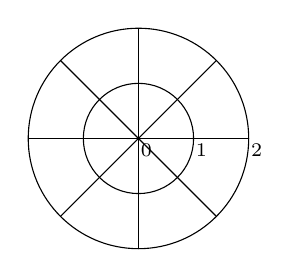
\begin{tikzpicture}[font=\scriptsize,scale=0.7]
            \draw (0,0) circle(1);
            \draw (0,0) circle(2);
            \foreach \i in {0,45,...,315} {
                    \draw (0,0) -- (\i:2);
                }
            \foreach \i in {0,1,2} {
                    \node[below,shift={(0.1,0.05)}] at (\i,0) {$\i$};
                }
        \end{tikzpicture}
        \hspace*{1cm}
    \end{center}
}
\usetikzlibrary{patterns}
\newcommand{\polarcoordinatetheta}{
    \begin{center}
        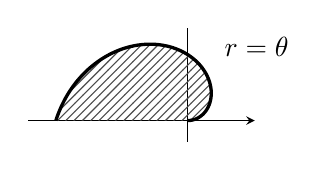
\begin{tikzpicture}
            \begin{axis}[
                    scale=0.42,
                    axis lines=middle,
                    y axis line style={-},
                    xmin=-3.8, xmax=1.6,
                    ymin=-0.5, ymax=2.2,
                    ticks=none,
                    axis equal image
                ]
                \addplot[
                    domain=0:pi,
                    samples=100,
                    pattern=north east lines,  % Hatching pattern
                    pattern color=black!70,
                    draw=none
                ]
                (
                {x*cos(deg(x))},
                {x*sin(deg(x))}
                )
                \closedcycle;
                \addplot[
                    domain=0:pi,
                    samples=100,
                    very thick,
                    black
                ]
                (
                {x*cos(deg(x))},
                {x*sin(deg(x))}
                );
            \end{axis}
            \node at (2.9, 1.2) {$r = \theta$};
        \end{tikzpicture}
        \hspace*{2.7cm}
    \end{center}
}
\newcommand{\polarcoordinatesintwotheta}{
    \begin{center}
        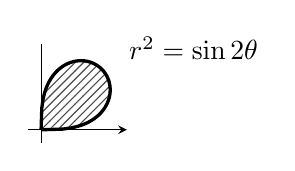
\begin{tikzpicture}
            \begin{axis}[
                    scale=0.22,
                    axis lines=middle,
                    y axis line style={-},
                    x=1cm, y=1cm,
                    xmin=-0.15, xmax=1,
                    ymin=-0.15, ymax=1,
                    ticks=none,
                    axis equal image
                ]
                \addplot[
                    domain=0:pi,
                    samples=100,
                    pattern=north east lines,  % Hatching pattern
                    pattern color=black!70,
                    draw=none
                ]
                (
                {sqrt(sin(deg(2*x))) * cos(deg(x))},
                {sqrt(sin(deg(2*x))) * sin(deg(x))}
                )
                \closedcycle;
                \addplot[
                    domain=0:pi,
                    samples=101,
                    very thick,
                    black
                ]
                (
                {sqrt(sin(deg(2*x))) * cos(deg(x))},
                {sqrt(sin(deg(2*x))) * sin(deg(x))}
                );
            \end{axis}
            \node at (2.1, 1.2) {$r^2 = \sin 2 \theta$};
        \end{tikzpicture}
        \hspace*{2.7cm}
    \end{center}
}

\begin{document}

\vspace*{44pt}
\enlargethispage{44pt}
\makeheading{ข้อสอบปลายภาค วิชา 2301207 Calculus III ปีการศึกษา 2568}

\bigskip

\begin{question}
    \item {} % 1
    \qmark{10} จงตอบคำถามเกี่ยวกับอินทิกรัลสองชั้นในพิกัดเชิงขั้ว
    \begin{question}
        \item กำหนดให้ $R$ เป็นบริเวณในครึ่งระนาบบนซึ่งอยู่ระหว่างวงกลมรัศมี $1$ และ $2$ หน่วยรอบจุดกำเนิด
        \begin{enumerate}[label=(\alph*),itemsep=12pt,topsep=5pt]
            \everymath={\displaystyle}
            \item จงร่างกราฟและ\uline{แรเงา}บริเวณ $R$ พร้อมทั้งเขียนบริเวณ $R$ ในพิกัดเชิงขั้ว

                  \medskip
                  \begin{minipage}{0.36\textwidth}
                      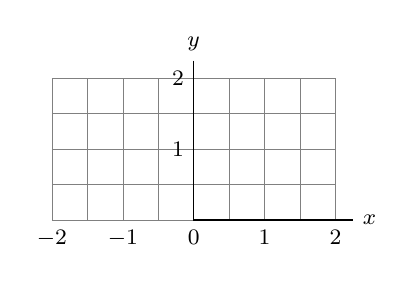
\begin{tikzpicture}[font=\footnotesize,scale=0.9]
                          \draw[help lines,xstep=0.5,ystep=0.5] (-2, 2) grid (2, 0);
                          \draw (0, 2.25) node[above]{$y$} |- (2.25, 0) node[right]{$x$};
                          \foreach \i in {1, 2} {
                                  \node[left] at (0, \i) {$\i$};
                              }
                          \foreach \i in {-2,...,2} {
                                  \node[below] at (\i, 0) {$\i$};
                              }
                      \end{tikzpicture}
                  \end{minipage}
                  \begin{minipage}{0.36\textwidth}
                      \vspace*{-1.6em}
                      \begin{align*}
                          R = \bigl\{ (r, \theta) \mid \  & \ansboxi{0.7cm} \leq r \leq \ansboxi{0.7cm},              \\
                                                          & \ansboxi{0.7cm} \leq \theta \leq \ansboxi{0.7cm}\,\bigr\}
                      \end{align*}
                  \end{minipage}

            \item $\iint\limits_R 1 \, d A = \ansbox$

            \item $\iint\limits_R \frac 1 {\sqrt{x^2 + y^2}} \, d A = \ansbox$

            \item $\iint\limits_R \sqrt{x^2 + y^2} \, d A = \ansbox$
        \end{enumerate}

        \vspace{2em}

        \item กำหนด $D$ เป็นบริเวณภายในครึ่งวงกลม $x = \displaystyle\sqrt{2y - y^2}$
        \begin{enumerate}[label=(\alph*),itemsep=12pt,topsep=5pt]
            \everymath={\displaystyle}
            \item จงร่างกราฟและ\uline{แรเงา}บริเวณ $D$ พร้อมทั้งเขียนบริเวณ $D$ ในพิกัดเชิงขั้ว

                  \medskip
                  \begin{minipage}{0.16\textwidth}
                      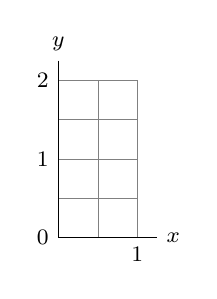
\begin{tikzpicture}[font=\footnotesize]
                          \draw[help lines,xstep=0.5,ystep=0.5] (0, 2) grid (1, 0);
                          \draw (0, 2.25) node[above]{$y$} |- (1.25, 0) node[right]{$x$};
                          \foreach \i in {0, 1, 2} {
                                  \node[left] at (0, \i) {$\i$};
                              }
                          \node[below] at (1, 0) {$1$};
                      \end{tikzpicture}
                  \end{minipage}
                  \begin{minipage}{0.46\textwidth}
                      \vspace*{-1.6em}
                      \begin{align*}
                          D = \bigl\{ (r, \theta) \mid \  & \ansboxi{0.7cm} \leq r \leq \ansboxi{1.4cm},              \\
                                                          & \ansboxi{0.7cm} \leq \theta \leq \ansboxi{0.7cm}\,\bigr\}
                      \end{align*}
                  \end{minipage}

            \item $\int_0^2 \int_0^{\sqrt{2y - y^2}} 1 \, d x \, d y = \ansbox$

            \item $\int_0^2 \int_0^{\sqrt{2y - y^2}} \frac 1 {\sqrt{x^2 + y^2}} \, d x \, d y = \ansbox$

            \item $\int_0^2 \int_0^{\sqrt{2y - y^2}} \frac {(x^2 + y^2)^{3/2}} {y^2} \, d x \, d y = \ansbox$
        \end{enumerate}
    \end{question}

    \pagebreak

    \item {} % 2
    \qmark{10} จงตอบคำถามเกี่ยวกับอินทิกรัลสามชั้นในพิกัดฉาก
    \begin{question}
        \everymath={\displaystyle}
        \item กำหนดให้ $B = [0, 1] \times [0, 1] \times [0, 1]$ \\[1em]
        $\iiint\limits_B x y^2 z^3 \, d V = \ansboxs \qquad \iiint\limits_B (x + y^2 + z^3) \, d V = \ansboxs$

        \vspace{2.8em}

        \item ให้ $E = \{(x, y, z) \mid 0 \leq x \leq y \leq z \leq 1\}$ \\[.5em]
        จงระบุขอบเขตของ $x, y, z$ สำหรับอินทิกรัลซ้อนของ $\iiint\limits_E f(x, y, z) \, d V$ ตาม\uline{ลำดับการอินทิเกรต}ที่กำหนดให้

        \def\tb#1{$\ansboxi{0.9cm} \leq #1 \leq \ansboxi{0.9cm}$}
        \begin{tabbing}
            $dx \, dy \, dz$\ : \quad \= $0 \leq z \leq 1$, \quad \= \tb{y}, \quad \= \tb{x} \\[0.8em]
            $dy \, dx \, dz$\ : \quad \> $0 \leq z \leq 1$, \quad \> \tb{x}, \quad \> \tb{y} \\[0.8em]
            $dz \, dy \, dx$\ : \quad \> $0 \leq x \leq 1$, \quad \> \tb{y}, \quad \> \tb{z} \\[0.8em]
            $dx \, dz \, dy$\ : \quad \> $0 \leq y \leq 1$, \quad \> \tb{z}, \quad \> \tb{x}
        \end{tabbing}

        \vspace{1.8em}

        \item ให้ $D$ เป็นบริเวณในระนาบ $xy$ ซึ่งปิดล้อมด้วยแกน $x$, เส้นตรง $x = 1$ และเส้นตรง $y = x$ \\
        ให้ $S$ เป็นทรงตันที่อยู่เหนือบริเวณ $D$ และอยู่ใต้ระนาบ $z = y$

        \medskip
        \begin{enumerate}[label=(\alph*),itemsep=15pt,topsep=5pt]
            \item จงเขียนอินทิกรัลสามชั้นในรูปอินทิกรัลซ้อนที่มีลำดับเป็น $dz \, dy \, dx$ \\[1em]
                  $\displaystyle \iiint\limits_S f(x, y, z) \, d V = \ansboxi{9.5cm}$

            \item ทรงตัน $S$ มีปริมาตร \ansboxs ลูกบาศก์หน่วย

                  \bigskip
            \item กำหนดให้ทรงตัน $S$ มีฟังก์ชันความหนาแน่น $f(x, y, z) = x$ กิโลกรัมต่อลูกบาศก์หน่วย \\[.5em]
                  ทรงตัน $S$ มีมวล \ansboxs กิโลกรัม และจุดศูนย์กลางมวลมี\uline{พิกัด $x$} เท่ากับ \ansboxs
        \end{enumerate}
    \end{question}

    \pagebreak

    \item {} % 3
    \qmark{10} กำหนดให้ทรงตัน $E$ เป็นโดเมนการอินทิเกรตของ $\displaystyle\int_0^1\int_x^1\int_0^{1-y^2} f(x, y, z) \, dz \, dy \, dx$
    \begin{question}
        \item จงร่างกราฟและ\uline{แรเงา}ภาพฉาย (projection) ของทรงตัน $E$ บนระนาบ $xy$, $yz$ และ $xz$ ตามลำดับ

        \bigskip
        \begin{minipage}{0.28\textwidth}
            \begin{tikzpicture}[font=\footnotesize,scale=3]
                \draw[help lines,xstep=0.25,ystep=0.25] (0, 1) grid (1, 0);
                \draw (0, 1.1) node[above]{$y$} |- (1.1, 0) node[right]{$x$};
                \node[left] at (0, 0.5) {$\frac12$};
                \node[left] at (0, 1) {$1$};
                \node[below left] at (0, 0) {$0$};
                \node[below] at (0.5, 0) {$\frac12$};
                \node[below] at (1, 0) {$1$};
                \node at (0.5, 1.15) {\normalsize\textbf{ระนาบ} $xy$};
            \end{tikzpicture}
        \end{minipage}
        \begin{minipage}{0.28\textwidth}
            \begin{tikzpicture}[font=\footnotesize,scale=3]
                \draw[help lines,xstep=0.25,ystep=0.25] (0, 1) grid (1, 0);
                \draw (0, 1.1) node[above]{$z$} |- (1.1, 0) node[right]{$y$};
                \node[left] at (0, 0.5) {$\frac12$};
                \node[left] at (0, 1) {$1$};
                \node[below left] at (0, 0) {$0$};
                \node[below] at (0.5, 0) {$\frac12$};
                \node[below] at (1, 0) {$1$};
                \node at (0.5, 1.15) {\normalsize\textbf{ระนาบ} $yz$};
            \end{tikzpicture}
        \end{minipage}
        \begin{minipage}{0.28\textwidth}
            \begin{tikzpicture}[font=\footnotesize,scale=3]
                \draw[help lines,xstep=0.25,ystep=0.25] (0, 1) grid (1, 0);
                \draw (0, 1.1) node[above]{$z$} |- (1.1, 0) node[right]{$x$};
                \node[left] at (0, 0.5) {$\frac12$};
                \node[left] at (0, 1) {$1$};
                \node[below left] at (0, 0) {$0$};
                \node[below] at (0.5, 0) {$\frac12$};
                \node[below] at (1, 0) {$1$};
                \node at (0.5, 1.15) {\normalsize\textbf{ระนาบ} $xz$};
            \end{tikzpicture}
        \end{minipage}

        \vspace{2.5em}

        \item จงระบุขอบเขตของ $x, y, z$ เมื่อ\uline{เปลี่ยนลำดับการอินทิเกรต}ของ $\displaystyle\int_0^1\int_x^1\int_0^{1-y^2} f(x, y, z) \, dz \, dy \, dx$ \\
        ตามลำดับที่กำหนดให้ต่อไปนี้

        \medskip
        \def\tb#1{$\ansboxi{0.9cm} \leq #1 \leq \ansboxi{1.6cm}$}
        \begin{tabbing}
            $dz \, dx \, dy$\ : \quad \= $0 \leq y \leq 1$, \quad \= $0 \leq x \leq \ansboxi{1.6cm}$, \quad \= \tb{z} \\[0.8em]
            $dx \, dz \, dy$\ : \quad \> $0 \leq y \leq 1$, \quad \> $0 \leq z \leq \ansboxi{1.6cm}$, \quad \> \tb{x} \\[0.8em]
            $dx \, dy \, dz$\ : \quad \> $0 \leq z \leq 1$, \quad \> $0 \leq y \leq \ansboxi{1.6cm}$, \quad \> \tb{x} \\[0.8em]
            $dy \, dz \, dx$\ : \quad \> $0 \leq x \leq 1$, \quad \> $0 \leq z \leq \ansboxi{1.6cm}$, \quad \> \tb{y} \\[0.8em]
            $dy \, dx \, dz$\ : \quad \> $0 \leq z \leq 1$, \quad \> $0 \leq x \leq \ansboxi{1.6cm}$, \quad \> \tb{y}
        \end{tabbing}

        \vspace{2.5em}

        \item จงหาค่า $\displaystyle\int_0^1\int_x^1\int_0^{1-y^2} \frac {\sqrt{z}} {1 - z - x\sqrt{1 - z}} \, dz \, dy \, dx$ โดยการเปลี่ยนลำดับการอินทิเกรต \\[2em]
        ลำดับการอินทิเกรตที่เหมาะสมในการหาค่าคือ \ansboxi{2.3cm} \quad ทำให้ได้ค่าอินทิกรัล $= \ansboxs$
    \end{question}

    \pagebreak

    \item {} % 4
    \qmark{10} จงตอบคำถามเกี่ยวกับอินทิกรัลสามชั้นในพิกัดทรงกระบอกและพิกัดทรงกลม

    \medskip
    \begin{question}
        \everymath={\displaystyle}
        \item ให้ $S$ เป็นทรงตัน\uline{ภายใน}กรวย $z = \sqrt{x^2 + y^2}$ และ\uline{ภายใน}พาราโบลอยด์ $z = 2 - x^2 - y^2$
        \begin{enumerate}[label=(\alph*),itemsep=16pt,topsep=5pt]
            \item กรวย $z = \sqrt{x^2 + y^2}$ มีสมการในพิกัดทรงกระบอกเป็น \ansboxl

            \item พาราโบลอยด์ $z = 2 - x^2 - y^2$ มีสมการในพิกัดทรงกระบอกเป็น \ansboxl

            \item ในพิกัดทรงกระบอก \mbox{$S = \bigl\{(r, \theta, z) \mid 0 \leq \theta \leq 2\pi,\ 0 \leq r \leq \ansboxi{0.6cm},\ \ansboxi{0.6cm} \leq z \leq \ansboxi{1.6cm}\,\bigr\}$}

            \item ทรงตัน $S$ มีปริมาตร \ansbox ลูกบาศก์หน่วย

                  \bigskip
            \item ถ้าทรงตัน $S$ มีฟังก์ชันความหนาแน่น $f(r, \theta, z) = 2 + \cos\theta$ กิโลกรัมต่อลูกบาศก์หน่วย \\[.5em]
                  แล้วทรงตัน $S$ มีมวล \ansbox กิโลกรัม
        \end{enumerate}

        \vspace{3.5em}

        \item ให้ $T$ เป็นทรงตัน\uline{ภายนอก}กรวย $z = \sqrt{x^2 + y^2}$ และ\uline{ภายใน}ทรงกลม $x^2 + y^2 + z^2 = 2z$
        \begin{enumerate}[label=(\alph*),itemsep=16pt,topsep=5pt]
            \item กรวย $z = \sqrt{x^2 + y^2}$ มีสมการในพิกัดทรงกลมเป็น \ansboxl

            \item ทรงกลม $x^2 + y^2 + z^2 = 2z$ มีสมการในพิกัดทรงกลมเป็น \ansboxl

            \item ในพิกัดทรงกลม \mbox{$T = \bigl\{(\rho, \theta, \phi) \mid 0 \leq \theta \leq 2\pi,\ \ansboxi{0.6cm} \leq \phi \leq \ansboxi{0.6cm},\ 0 \leq \rho \leq \ansboxi{1.6cm}\,\bigr\}$}

            \item ทรงตัน $T$ มีปริมาตร \ansbox ลูกบาศก์หน่วย

                  \bigskip
            \item ถ้าทรงตัน $T$ มีฟังก์ชันความหนาแน่น $f(\rho, \theta, \phi) = 2 + \cos\theta$ กิโลกรัมต่อลูกบาศก์หน่วย \\[.5em]
                  แล้วทรงตัน $T$ มีมวล \ansbox กิโลกรัม
        \end{enumerate}
    \end{question}

    \pagebreak

    \item {} % 5
    \qmark{10} จงตอบคำถามเกี่ยวกับอินทิกรัลสามชั้นในพิกัดทรงกระบอกและพิกัดทรงกลม

    \medskip
    \begin{question}
        \everymath={\displaystyle}
        \item ให้ $S$ เป็นโดเมนการอินทิเกรตของ $\int_{-1}^1 \int_{-\sqrt{1-y^2}}^{\sqrt{1-y^2}} \int_{\sqrt{x^2+y^2}}^1 f(x, y, z) \, dz \, dx \, dy$
        \begin{enumerate}[label=(\alph*),itemsep=12pt,topsep=5pt]
            \item ในพิกัดทรงกระบอก $S = \bigl\{(r, \theta, z) \mid 0 \leq \theta \leq 2\pi,\ 0 \leq r \leq \ansboxi{0.6cm},\ \ansboxi{0.6cm} \leq z \leq \ansboxi{0.6cm}\,\bigr\}$

            \item ในพิกัดทรงกลม \mbox{$S = \bigl\{(\rho, \theta, \phi) \mid 0 \leq \theta \leq 2\pi,\ \ansboxi{0.6cm} \leq \phi \leq \ansboxi{0.6cm},\ 0 \leq \rho \leq \ansboxi{1.6cm}\,\bigr\}$}

            \item $\iiint\limits_S 1 \, dV = \ansboxi{2.4cm}$

            \item $\iiint\limits_S \sqrt{x^2 + y^2} \, dV = \ansboxi{2.4cm}$

            \item $\iiint\limits_S \sqrt{x^2 + y^2 + z^2} \, dV = \ansboxi{3.5cm}$
        \end{enumerate}

        \vspace{4em}

        \item ให้ $T$ เป็นโดเมนการอินทิเกรตของ $\int_{-1}^1 \int_{-\sqrt{1-x^2}}^{\sqrt{1-x^2}} \int_0^{\sqrt{1-x^2-y^2}} f(x, y, z) \, dz \, dy \, dx$
        \begin{enumerate}[label=(\alph*),itemsep=12pt,topsep=5pt]
            \item ในพิกัดทรงกระบอก \mbox{$T = \bigl\{(r, \theta, z) \mid 0 \leq \theta \leq 2\pi,\ 0 \leq r \leq \ansboxi{0.6cm},\ 0 \leq z \leq \ansboxi{1.6cm}\,\bigr\}$}

            \item ในพิกัดทรงกลม $T = \bigl\{(\rho, \theta, \phi) \mid 0 \leq \theta \leq 2\pi,\ \ansboxi{0.6cm} \leq \phi \leq \ansboxi{0.6cm},\ 0 \leq \rho \leq \ansboxi{0.6cm}\,\bigr\}$

            \item $\iiint\limits_T 1 \, dV = \ansboxi{2.4cm}$

            \item $\iiint\limits_T \sqrt{x^2 + y^2} \, dV = \ansboxi{2.4cm}$

            \item $\iiint\limits_T \sqrt{1 - x^2 - y^2} \, dV = \ansboxi{2.4cm}$
        \end{enumerate}
    \end{question}

    \pagebreak

    \item {} % 6
    \qmark{6} ให้อินทิกรัล $\displaystyle I = \iint\limits_R \cos \left[\left(\tfrac{x^2}{4} + y^2\right) \pi\right] dA$
    โดยที่ $R$ คือบริเวณภายในวงรี $x^2 + 4y^2 = 1$ \\ ที่อยู่จตุภาคที่ $1$
    กล่าวคือ $R = \left\{(x, y) \mid x^2 + 4y^2 \leq 1,\ x \geq 0,\ y \geq 0\right\}$

    \vspace{2em}
    เมื่อเปลี่ยนตัวแปรให้ $x = 2u \cos v$ และ $y = u \sin v$ ที่มี $u \geq 0$ และ $0 \leq v \leq 2\pi$ จะได้
    \[
        I = \iint\limits_S f(u, v) \left|\frac{\partial(x, y)}{\partial(u, v)}\right| \, du \, dv
    \]
    \begin{question}[itemsep=16pt]
        \item \qmark{2} เมื่อหาขอบเขตของบริเวณ $S$ บนระนาบ $uv$ \\[.5em]
        จะได้ขอบเขตของตัวแปร $\ansboxi{0.7cm} \leq u \leq \ansboxi{0.7cm}$\, และ \,$\ansboxi{0.7cm} \leq v \leq \ansboxi{0.7cm}$

        \item \qmark{2} $f(u, v) = \ansboxi{3.6cm}$ และ $\dfrac{\partial(x, y)}{\partial(u, v)} = \ansboxi{3.6cm}$

        \item \qmark{2} เมื่อคำนวณหาค่าอินทิกรัล จะได้ $I = \ansboxi{3.6cm}$
    \end{question}

    \vspace{5.5em}

    \item {} % 7
    \qmark{4} เมื่อใช้การเปลี่ยนตัวแปรหาค่าอินทิกรัล $\displaystyle I = \iint\limits_R 2x e^{x^2 - 4y^2} \, dA$
    บนบริเวณ $R$ ที่ปิดล้อมด้วย $x + 2y = 0$, $x + 2y = 2$, $x - 2y = 0$ และ $x - 2y = 2$
    โดยให้ $u = x + 2y$ และ $v = x - 2y$ จะได้
    \[
        I = \iint\limits_S f(u, v) \left|\frac{\partial(x, y)}{\partial(u, v)}\right| \, du \, dv
    \]
    \begin{question}[itemsep=16pt]
        \item \qmark{2} $f(u, v) = \ansboxi{3.6cm}$ และ $\dfrac{\partial(x, y)}{\partial(u, v)} = \ansboxi{3.6cm}$

        \item \qmark{2} เมื่อคำนวณหาค่าอินทิกรัล จะได้ $I = \ansboxi{3.6cm}$
    \end{question}

    \pagebreak

    \item {} % 8
    \qmark{10} จงหาค่าอินทิกรัลตามเส้นต่อไปนี้ (เติมเฉพาะคำตอบในรูปสำเร็จ ไม่ต้องแสดงวิธีทำ)
    \begin{question}[itemsep=2.6cm]
        \item \qmark{2} ให้ $C$ เป็นส่วนของวงกลม $x^2 + y^2 = 4$ ที่อยู่ในจตุภาคที่ $1$ ($x \geq 0$, $y \geq 0$) \\[.5em]
        จะได้ $\displaystyle \int\limits_C x^2 y \, ds = \ansboxi{3.6cm}$

        \item \qmark{2} ให้ $C$ เป็นส่วนของเส้นตรง ที่ลากจากจุด $(1,0)$ ไปยัง $(0,1)$ \\[.5em]
        จะได้ $\displaystyle \int\limits_C (x + y^2) \, dx = \ansboxi{3.6cm}$

        \item \qmark{2} ให้ $C$ เป็นเส้นโค้งที่กำหนดโดยสมการ $x = 3 \cos t$, $y = 3 \sin t$, $z = 4t$ สำหรับ $0 \leq t \leq \pi$ \\[.5em]
        จะได้ $\displaystyle \int\limits_C e^z \, ds = \ansboxi{3.6cm}$

        \item \qmark{2} ให้ $C$ เป็นเส้นโค้งที่กำหนดโดยสมการเวกเตอร์ $\mathbf{r}(t) = \langle t^3, t^2, t \rangle$ สำหรับ $0 \leq t \leq 1$ \\[.5em]
        จะได้ $\displaystyle \int\limits_C x e^{yz^3} \, dy = \ansboxi{3.6cm}$

        \item \qmark{2} ให้ $\mathbf{F}(x, y) = \langle 2y, x^2 + y^2 \rangle$ และ $\mathbf{r}(t) = \langle \sqrt{t}, t \rangle$ สำหรับ $0 \leq t \leq 1$ \\[.5em]
        จะได้ $\displaystyle \int\limits_C \mathbf{F} \cdot d\mathbf{r} = \ansboxi{3.6cm}$
    \end{question}

    \pagebreak

    \item {} % 9
    \qmark{4} (แสดงวิธีทำ) จงหางานที่กระทำโดยสนามแรง $\mathbf{F}(x, y, z) = \langle 2x - y, 2y - z, 2z - x \rangle$
    บนวัตถุที่เคลื่อนที่เป็นแนวเส้นตรง จากจุด $(1, 1, 1)$ ไปยังจุด $(3, 4, 5)$

    \medskip
    \textbf{วิธีทำ:}

    \vspace{21em}

    \item {} % 10
    \qmark{6} ให้เส้นลวดมีลักษณะเป็นเส้นโค้งที่กำหนดโดยสมการเวกเตอร์ $\mathbf{r}(t) = \langle \cos t, \sin t, t \rangle$ สำหรับ $0 \leq t \leq 1$
    และเส้นลวดมีความหนาแน่น $\rho(x, y, z) = x^2 + y^2 + z^2$ จงหาค่าต่อไปนี้
    \begin{question}
        \item \qmark{2} ความยาวของเส้นลวด $L = \ansboxi{3.6cm}$

        \item \qmark{2} มวลของเส้นลวด $m = \ansboxi{3.6cm}$

        \item \qmark{2} ถ้าให้ $(\bar{x}, \bar{y}, \bar{z})$ เป็นจุดศูนย์กลางมวลของเส้นลวดนี้ \\[.5em]
        จะได้ $\bar{z} = \ansboxi{3.6cm}$
    \end{question}

    \pagebreak

    \item {} % 11
    \qmark{6} จงหาค่าต่อไปนี้โดยเติมคำตอบลงในช่องว่างที่กำหนดให้
    \begin{question}
        \item \qmark{2} ให้ $f(x, y) = xy^2$ และ $C$ เป็นเส้นโค้งที่กำหนดโดยสมการ $x = 1 + 2 \cos(\frac{\pi t}{2})$
        และ $y = 2 + 2 \sin(\frac{\pi t}{2})$ สำหรับ $0 \leq t \leq 1$ \\[.5em]
        จะได้ $\displaystyle \int\limits_C \nabla f \cdot d\mathbf{r} = \ansboxi{3.6cm}$

        \vspace{3.8em}

        \item ให้ $\mathbf{F}(x, y) = \langle -\dfrac{y^2}{x^2}, \dfrac{2y}{x} - 1 \rangle$ \textbf{เป็นสนามอนุรักษ์}
        ที่มี $f(x, y)$ เป็น \textbf{ฟังก์ชันศักย์} และ $f(1, -1) = 3$
        \begin{enumerate}[label=(\alph*),itemsep=12pt,topsep=25pt]
            \item \qmark{2} จะได้ $f(x, y) = \ansboxi{7cm}$

                  \vspace{4.2em}
            \item \qmark{2} ให้ $C$ เป็นส่วนของเส้นตรงที่ลากจาก $(1, -1)$ ไปยัง $(3, 3)$ \\[.5em]
                  จะได้ $\displaystyle \int\limits_C \mathbf{F} \cdot d\mathbf{r} = \ansboxi{3.6cm}$
        \end{enumerate}
    \end{question}

    \vspace{3.1em}

    \item {} % 12
    \qmark{4} ให้ $\mathbf{F}(x, y, z) = \langle e^{-yz}, -xz e^{-yz}, -xy e^{-yz} \rangle = \nabla f(x, y, z)$ เป็นสนามอนุรักษ์
    \begin{question}
        \item \qmark{2} ถ้า $f(1, -2, 0) = 5$ จะได้ $f(x, y, z) = \ansboxi{6.8cm}$

        \vspace{3.8em}
        \item \qmark{2} ให้เส้นโค้ง $C$ มีสมการเวกเตอร์ $\mathbf{r}(t) = \langle \sqrt{2t^2 + 1}, t - 2, 2t^2 \rangle$ สำหรับ $0 \leq t \leq 2$ \\[.5em]
        จะได้ $\displaystyle \int\limits_C \mathbf{F} \cdot d\mathbf{r} = \ansboxi{3.6cm}$
    \end{question}

    \pagebreak

    \item {} % 13
    \qmark{5} (แสดงวิธีทำ) ใช้ทฤษฎีบทของกรีนหาค่าของ $\displaystyle \oint\limits_C y^3 \, dx - xy^2 \, dy$
    เมื่อ $C$ คือวงกลม $x^2 + y^2 = 4$ มีทิศทางทวนเข็มนาฬิกา (\textbf{สูตร:} $\sin^2 \theta = \dfrac{1 - \cos 2\theta}{2}$, $\cos^2 \theta = \dfrac{1 + \cos 2\theta}{2}$)

    \medskip
    \textbf{วิธีทำ:}

    \vspace{16em}

    \item {} % 14
    \qmark{5} จงหาค่าอินทิกรัลตามเส้นต่อไปนี้ โดยเติมเฉพาะคำตอบตามที่โจทย์ถาม (ไม่ต้องแสดงวิธีทำ)
    \begin{question}
        \item \qmark{3} ให้ $C$ เป็นสามเหลี่ยมที่มีจุดยอด $(0, 0)$, $(1, 0)$ และ $(0, 1)$ และมีทิศทวนเข็มนาฬิกา \\[.5em]
        จะได้ $\displaystyle \oint\limits_C x^2 y \, dx + \tan^{-1} y \, dy = \underset{\text{(ตอบในรูปอินทิกรัลซ้อนตามทฤษฎีบทของกรีน โดยใช้ลำดับ $dy \, dx$)}}{\boxed{\vphantom{\dfrac{\dfrac12}{\dfrac12}}\phantom{\hspace*{6.7cm}}}}$ \\[.5em]
        $= \underset{\text{(ตอบค่าอินทิกรัลในรูปเศษส่วนอย่างต่ำ)}}{\ansboxi{3.3cm}}$

        \item \qmark{2} ให้ $\mathbf{F}(x, y) = \langle x e^{x^2} - 2y, 3x - y^3 \rangle$
        และ $C$ เป็นเส้นขอบของบริเวณ $D$ ที่มีทิศทวนเข็มนาฬิกา
        ซึ่งบริเวณ $D$ มีพื้นที่ $6$ ตารางหน่วย \\[.5em]
        จะได้ $\displaystyle \oint\limits_C \mathbf{F} \cdot d\mathbf{r} = \ansboxi{3.6cm}$
    \end{question}
\end{question}

\end{document}